\documentclass{beamer}

\usepackage{listings}
\usepackage{color}
\usepackage{hyperref}

\usepackage[T1]{fontenc}
\usepackage{textcomp}
\usepackage{upquote}

% Default fixed font does not support bold face
\DeclareFixedFont{\ttb}{T1}{txtt}{bx}{n}{10} % for bold
\DeclareFixedFont{\ttm}{T1}{txtt}{m}{n}{10}  % for normal

% Custom colors
\usepackage{color}
\definecolor{deepblue}{rgb}{0,0,0.5}
\definecolor{deepred}{rgb}{0.6,0,0}
\definecolor{deepgreen}{rgb}{0,0.5,0}
\definecolor{shadecolor}{rgb}{1, 0.9, 0.3}

\usepackage{listings}
\lstset{basicstyle=\ttfamily,
  showstringspaces=false,
  commentstyle=\color{red},
  keywordstyle=\color{blue}
}

% Python style for highlighting
\newcommand\pythonstyle{\lstset{
language=Python,
basicstyle=\ttm,
otherkeywords={self},             % Add keywords here
keywordstyle=\ttb\color{deepblue},
%emph={MyClass,__init__},          % Custom highlighting
emphstyle=\ttb\color{deepred},    % Custom highlighting style
stringstyle=\color{deepgreen},
frame=tb,                         % Any extra options here
showstringspaces=false,            % 
upquote=True,
columns=fullflexible,
basicstyle=\ttfamily
}}


% Python environment
\lstnewenvironment{code}[1][]
{
%\begin{small}
\pythonstyle
\lstset{#1}
%\end{small}
}
{}


\begin{document}

% Theory of objects. (maybe Inheritance. Design). Objects = methods plus attributes. Self. Calling methods via dot vs just calling functions.  __init__. private.

\begin{frame}
\frametitle{CS24420 \& MA25220 \& MT25220 \& MX35220 \& CSM0120}

\begin{center}
\begin{huge}
Lecture 13: Object-oriented code 
\end{huge}
\bigskip

Alexander Pitchford (agp1@aber.ac.uk)

\end{center}
\end{frame}

%---------------------------------------------------
\begin{frame}[fragile]
\frametitle{A World Full of Objects}
The world is full of objects:
\begin{itemize}
\item chairs
\item tables
\item buildings
\item planets
\item stars
\item washing machines
\end{itemize}

\end{frame}

%----------------------------------------------------
\begin{frame}[fragile]
\frametitle{Things}
The world also contains other things:
%SpeakerNote: Things that we would not usually call objects
\begin{itemize}
\item atoms
\item animals
\item people
\item bacteria
\item emotions
\item philosophical concepts
\end{itemize}
\pause
\bigskip
All these objects and things have characteristics,\\
% chairs have a number of legs
% plants have a mass and a radius
% washing machines have a model name
\smallskip
\pause
and possibly actions associated with them.
% either things they do or have done to them
% stars radiate
% washing machines wash clothes
% emotions can expressed
% philosophical concepts can be argued
\bigskip

\end{frame}

%----------------------------------------------------
\begin{frame}[fragile]
\frametitle{Object-oriented Programming}

\begin{itemize}
\item Naturally then we would like some way of representing these things in code.
\item In many computer programming languages objects and things can be represented by \emph{objects}.
\item Characteristics by \emph{attributes} or \emph{properties}.
\item Actions by \emph{methods}.
\item Languages that support this are called \emph{Object-Oriented},
\item or 'OO' for short.
\end{itemize}

\end{frame}

%----------------------------------------------------
\begin{frame}[fragile]
\frametitle{Outline}

\begin{itemize}
\item Objects in Python
\item Creating and using objects
\item Defining objects through classes
\item Class inheritance
\item Use of washing machine and people examples
\end{itemize}

\end{frame}

%----------------------------------------------------
\begin{frame}[fragile]
\frametitle{Objects in Python}
\begin{itemize}
\item Python is an Object-Oriented language.
% Not as OO as some others, like C++ or Java
% Many people happily write Python using module and functions 
% and rarely, if ever, write a custom class
\item Objects are everywhere in Python.
\item We have used objects in all the workshops.
\item All of these are objects:
\begin{itemize}
\item strings
\item modules
\item lists, dictionaries, numpy arrays
\item Exceptions
\end{itemize}
\item In fact all variables of all types.
\end{itemize}
% Switch to live demo:
% showing how strings have methods like upper() and lower()
% numpy has a __name__ attribute
% an Exception has a string representation
% numbers have a real and imaginary part
\begin{code}
"ABC".lower()
numpy.__name__
\end{code}
\end{frame}

%----------------------------------------------------
\begin{frame}[fragile]
\frametitle{Creating an Object}
\begin{itemize}
\item So we create objects all the time whenever we set a variable value.
\item These are examples of creating an object.
\end{itemize}

\begin{code}
myobj = ClassName()
mach1 = WashingMachine()
pfact = PeopleFactory()
\end{code}

\end{frame}

%----------------------------------------------------
\begin{frame}[fragile]
\frametitle{Creating an Object - with arguments}

\begin{itemize}
\item In the previous examples no arguments are given,
\item meaning that a generic object will be created -
\item Repeated calls will make identical objects.
\item Sometimes we create them with \emph{initialisation arguments}.
\item These generate objects with some attributes already set to specific values.
\end{itemize}

\begin{code}
myobj = ClassName(init_arg1, init_arg2)
mach1 = WashingMachine("Hotpoint WMFUG842G")
sam = Person("Sam Nicholls", 'male', 25, 1.6)
pstats = PersonalStatistics(meandmyfriends)
arr1 = numpy.array([1, 2], [3, 4]])
\end{code}
\end{frame}

%----------------------------------------------------
\begin{frame}[fragile]
\frametitle{Using Objects}
The attributes and methods of objects are all accessed using the dot '.'
\begin{itemize}
\item Setting attributes
\begin{code}
myobj.my_attribute = "some value"
mach1.model = "Hotpoint WMFUG842G"
sam.age = 26
\end{code}
\item Accessing attributes
\begin{code}
print("My attribute value is: " + myobj.my_attribute)
if mach1.detergent_avail:
\end{code}
\item Calling (or running) methods
\begin{code}
myobj.my_method(metharg1, metharg2)
mach1.wash()
pfact.generate_random_people(1000)
\end{code}
% Emphasize the brackets
\end{itemize}
\end{frame}

%----------------------------------------------------
\begin{frame}[fragile]
\frametitle{Classes}
\begin{itemize}
\item An object is a single \emph{instance} of a thing.
\item To produce many instances, we use a template, or, mould.
\item This template we call a \emph{class}
\item Each instance need not be identical.
\item It may have different characteristics - 
\begin{itemize}
\item different attribute values
\end{itemize}
\item But the same actions will be applicable -
\begin{itemize}
\item the same methods will be available
\end{itemize}
\end{itemize}
\end{frame}

%----------------------------------------------------
\begin{frame}[fragile]
\frametitle{Defining Objects through Classes}
\begin{itemize}
\item Defining your own custom objects is done through a \emph{class}
by using the \lstinline|class| statement.
\begin{code}
class MyClass(object):
  """MyClass does some interesting things"""
  # Everything indented at this level 
  # or beyond is part of the class
\end{code}
\item Note the naming convention: 'CapWords'.
%Explain that this is optional, so don't expect to see it everywhere
%but that they should use it
\item Note the \emph{inheritance} (explained later) from \lstinline|object|.
%Explain that this is optional, but that they should use it
\item Note the \emph{docstring}, which should explain what the class is for.
\end{itemize}
Note: we can make many instances of \lstinline|MyClass|. 
Each of which can have different attribute values,
but all instances will all be of the same \emph{class}.

\end{frame}

%----------------------------------------------------
\begin{frame}[fragile]
\frametitle{Methods}
\begin{itemize}
\item Methods are functions attached to the object.
\item Methods have a name and possibly arguments (or parameters).
\item The first argument should always be the \lstinline|self| variable.
% These are variables passed to the method
\item They are named, by convention, using lower case with underscores as separators, 
e.g. \lstinline|my_method|
\item They may return a value, but don't have to.
\end{itemize}
Methods are defined in the class:
\begin{code}
class MyClass(object):
  def my_method(self, testtarg1):
    """Do some work"""
    if self.my_attrib == testtarg1:
    	return "Success"
    else:
    	return "Fail"
\end{code}

\end{frame}

%----------------------------------------------------
\begin{frame}[fragile]
\frametitle{Use of self}
\begin{itemize}
\item Note the use of \lstinline|self| in the method.
\begin{code}
class MyClass(object):
  def my_method(self, testtarg1):
\end{code}
\item The \lstinline|self| variable points to the current instance - 
the object that called the method.
\item It should be the first argument of all methods.
\item It is passed automatically when the object method is called.
\begin{code}
myobj = MyClass()
ret = myobj.my_method(testthis)
\end{code}
\item This is equivalent
\begin{code}
myobj = MyClass()
ret = MyClass.my_method(myobj, testthis)
\end{code}
\end{itemize}

\end{frame}

%----------------------------------------------------
\begin{frame}[fragile]
\frametitle{Attributes}

\begin{itemize}
\item Attributes are variables attached to the object.
\item Attributes have a name and a value.
\item They are named, by convention, using lower case with underscores as separators, 
e.g. \lstinline|my_attrib|
\item Attributes are created when the value is set during the initialisation.
% which will be explained shortly
\item The methods will almost certainly use the attributes during their execution.
\item They are always referred to in the methods using the \lstinline|self| variable.
\end{itemize}
\begin{code}
class MyClass(object):
  def my_method(self, testtarg1):
    if self.my_attrib == testtarg1:
      # do something
\end{code}
\end{frame}

%----------------------------------------------------
\begin{frame}[fragile]
\frametitle{Class Initialisation}
\begin{itemize}
\item A class initialisation method is usually required.
\item It has to be called \lstinline|__init__|.
% mention that we will come back to this later
\item The first argument will be \lstinline|self|. 
\item There can be others, either required or optional (kwargs).
\item The method can define attributes by setting their values.
\item These can be hardcoded or based on the method arguments.
\end{itemize}
% Note self

\begin{code}
class MyClass(object):
  def __init__(self, initarg1, initarg2=None):
    """Initialise initarg1 and (optionally) initarg2"""
    self.attrib1 = initarg1
    if initarg2 is None:
      self.attrib2 = initarg2
    else:
      self.attrib2 = 0.0
    self.attrib3 = False
\end{code}

\end{frame}

%----------------------------------------------------
% Look at example inside of Spyder, this is here just in case
\begin{frame}[fragile]
\frametitle{Example - WashingMachine}
\begin{code}
class WashingMachine(object):
    """Machine for washing clothes"""
    dirty_words = ['dirty', 'filthy', 'grubby', 'soiled']
    wet_words = ['wet', 'damp', 'soggy', 'drenched']
    def __init__(self, model_name=None):
        """Initialise WashingMachine, optionally with model_name"""
        if model_name is None:
            self.model = 'generic washing machine'
        else:
            self.model = model_name
        self.contents = 'empty'
        self.detergent_avail = False
        self.fill_time = 1.0
        self.wash_time = 2.0
        self.spin_time = 1.0
\end{code}
\end{frame}

%----------------------------------------------------
\begin{frame}[fragile]
\frametitle{Example - WashingMachine}
\begin{code}
    def load(self, contents):
        """Load the machine with the contents"""
        self.contents = str(contents)
        
    def add_detergent(self):
        """Add some detergent to the machine"""
        self.detergent_avail = True
        
    def empty(self):
        """Remove the contents"""
        self.contents = 'empty'
\end{code}
\end{frame}

%----------------------------------------------------
\begin{frame}[fragile]
\frametitle{Example - WashingMachine}
Creating WashingMachine objects:
\begin{code}
genmach = WashingMachine()
hotpnt = WashingMachine("Hotpoint WMFUG842G")
bosch = WashingMachine(model_name="Bosch WAN28280GB")
\end{code}
\end{frame}

%----------------------------------------------------
\begin{frame}[fragile]
\frametitle{Private Attributes and Methods}

% Just talking about these, as they are likely to be encountered
% We are not going to be using these in the workshop
\begin{itemize}
\item In OO programming \emph{private} means 'internal use only'.
\item There is no implementation of 'private' in Python objects.
% As is found in some other OO languages
\item However, often class authors wish to imply privacy.
\item This is done starting the method or attribute name with a single underscore.
\begin{code}
class SomeClass(object):
  def _some_private_method(self):
    self._private_attrib = "some value"
\end{code}

\item You should avoid accessing them in your code.
\item Usage may change in future versions of the class.
\item They may disappear altogether.
\item We will not be using them in this course.
\end{itemize}

\end{frame}

%----------------------------------------------------
\begin{frame}[fragile]
\frametitle{Python 'system' Attributes and Methods}
\begin{itemize}
\item Python system internal, or \emph{magic}, attributes and methods are
named with double leading and trailing underscores.
\item You must \emph{not} name your attributes with double leading and trailing underscores!
\item You are likely to often use these magic methods.
\item We have come across two already \lstinline|__name__| and \lstinline|__init__|.
\item Some other useful ones are \lstinline|__str__| and \lstinline|__repr__|.
\item If you implement them in your class, then they define how the objects will be represented as string.
\item For instance when the object is printed.
\item There is an example in the workshop \lstinline|Person| class.
\end{itemize}
\end{frame}

%----------------------------------------------------
\begin{frame}[fragile]
\frametitle{Example - string representation}
\begin{code}
class MyClass(object):
  def __init__(self, obj_name):
    self.name = obj_name
  def __str__(self):
    return "{} of name {}".format(self.__class__.__name__, 
                              self.name)
                              
myobj = MyClass("foo")
print(myobj)

>>> MyClass of name foo

\end{code}
\end{frame}


%----------------------------------------------------
\begin{frame}[fragile]
\frametitle{Classification Systems}
\begin{itemize}
\item Often we can classify things hierarchically.
\begin{itemize}
\item 'Table' and 'Chair' both belong to a \emph{supertype} 'Furniture'.
\item Planets and Stars are both sub-types of CelestialBody
\item Salmon is a sub-type of Fish, which is in turn a sub-type of Animal
\item WasherDryer is a sub-type of Washing Machine.
\item Student and Lecturer are both sub-types of Person
\end{itemize}
\item Mathematically we could call some a 'subsets' of the other.
\end{itemize}

\end{frame}

%----------------------------------------------------
\begin{frame}[fragile]
\frametitle{Example Hierarchy}
% Find some Tree of Life image for here
% Maybe also the Standard Model
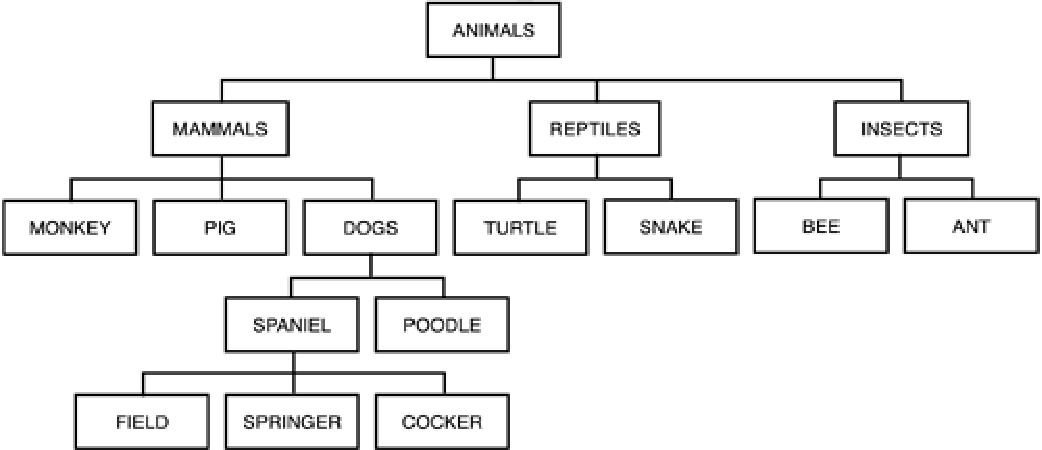
\includegraphics[width=10cm]{animal_hierarch.pdf}
\end{frame}

%----------------------------------------------------
\begin{frame}[fragile]
\frametitle{Inheritance}
% This is where the true power of OO programming resides
\begin{itemize}
\item Through \emph{inheritance} we can define classes in a hierarchical way.
\item A new class can inherit all the attributes and methods of its \emph{superclass}
\item This class is then called the \emph{subclass} of the \emph{superclass}
\begin{code}
  class MySubClass(TheSuperClass):
\end{code}
\item The superclass could be something that you wrote yourself,
\item or it could be something from Python's core or some other module.
\item This can be very powerful, as you can always use the subclass wherever the superclass is used.
\item For instance, one could subclass the numpy array, add some new functionality, 
but still use all the numpy methods that accept arrays.
% The numpy matrix is an example of this

\end{itemize}
% Superclasses and sub-classes
% overriding methods
% calling the superclass methods


\end{frame}

%----------------------------------------------------
\begin{frame}[fragile]
\frametitle{Overriding}
% overriding methods
% calling the superclass methods

\begin{itemize}
\item All the superclass methods are available to the subclass.
\item However, the function of these methods can be changed through \emph{overriding}.
\item To override a method one simply implements a new method in the subclass with the same name.
\item Often the subclass method wants to call the superclass method that it overrides,
\item particularly when overriding the \lstinline|__init__| method.
\begin{code}
  class MySubClass(TheSuperClass):
    def __init__(self, initarg)
      TheSuperClass.__init__(self, initarg)
      # subclass specific stuff here
\end{code}
\end{itemize}

\end{frame}

%----------------------------------------------------
\begin{frame}[fragile]
\frametitle{Example - WasherDryer}
\begin{code}
class WasherDryer(WashingMachine):
    """Machine for washing and drying clothes"""
    def __init__(self, model_name=None):
        WashingMachine.__init__(self)
        if model_name is None:
          self.model = 'generic washer dryer'
        self.dry_time = 1.0

    def dry(self):
        print("Drying...")
        time.sleep(self.dry_time)
        for ww in self.wet_words:
            if ww in self.contents:
                self.contents = \
                       self.contents.replace(ww, 'dry')
        print("Dry cycle finished")
        
\end{code}

\end{frame}

%----------------------------------------------------
\begin{frame}[fragile]
\frametitle{When to use Custom Objects}
\begin{itemize}
\item When there are many things with the same function and characteristics,
but different values for the characteristics.
\begin{itemize}
\item A data set, such as experimental output, is a good example.
\end{itemize}
\item When there is a hierarchy to the structure of function.
\end{itemize}

\end{frame}

%----------------------------------------------------
\begin{frame}[fragile]
\frametitle{Summary}
\begin{itemize}
\item Objects are everywhere in Python.
\item Objects are defined by templates called classes
\item Objects are created using the class.
\item Classes define the methods (functions) and attributes (characteristics) of the objects.
\item Classes can be defined in a hierarchy, each inheriting the methods and attributes of the parent.
\end{itemize}


\end{frame}

\end{document}